% =====================================================================
%  Fotos der Tauchsäge (Grundstellung und eingetaucht) mit nummerierten
%  Bedienelementen. Fotos: Oxensepp, Wikimedia Commons, CC BY-SA 3.0
%  (siehe bilder/QUELLEN.md). Koordinaten relativ zum jeweiligen Foto:
%  (0,0) unten links, (1,1) oben rechts.
%  Nummern wie in der Tabelle in einweisung_Kreissaege.tex
% =====================================================================
\begin{tikzpicture}[
    marke/.style={circle, draw=black, fill=white, line width=1pt,
      minimum size=5mm, inner sep=0pt, font=\small\bfseries},
    titel/.style={anchor=north west, fill=white, fill opacity=0.85,
      text opacity=1, font=\small\bfseries, inner sep=1.2mm}]
  % \nr{Nummer}{Position der Nummer}{Bauteil}
  \newcommand{\nr}[3]{%
    \draw[white, line width=2pt, line cap=round] (#2) -- (#3);
    \draw[black, line width=0.8pt] (#2) -- (#3);
    \fill[black] (#3) circle[radius=0.7mm];
    \node[marke] at (#2) {#1};}

  \node[anchor=south west, inner sep=0pt] (a) at (0,0)
    {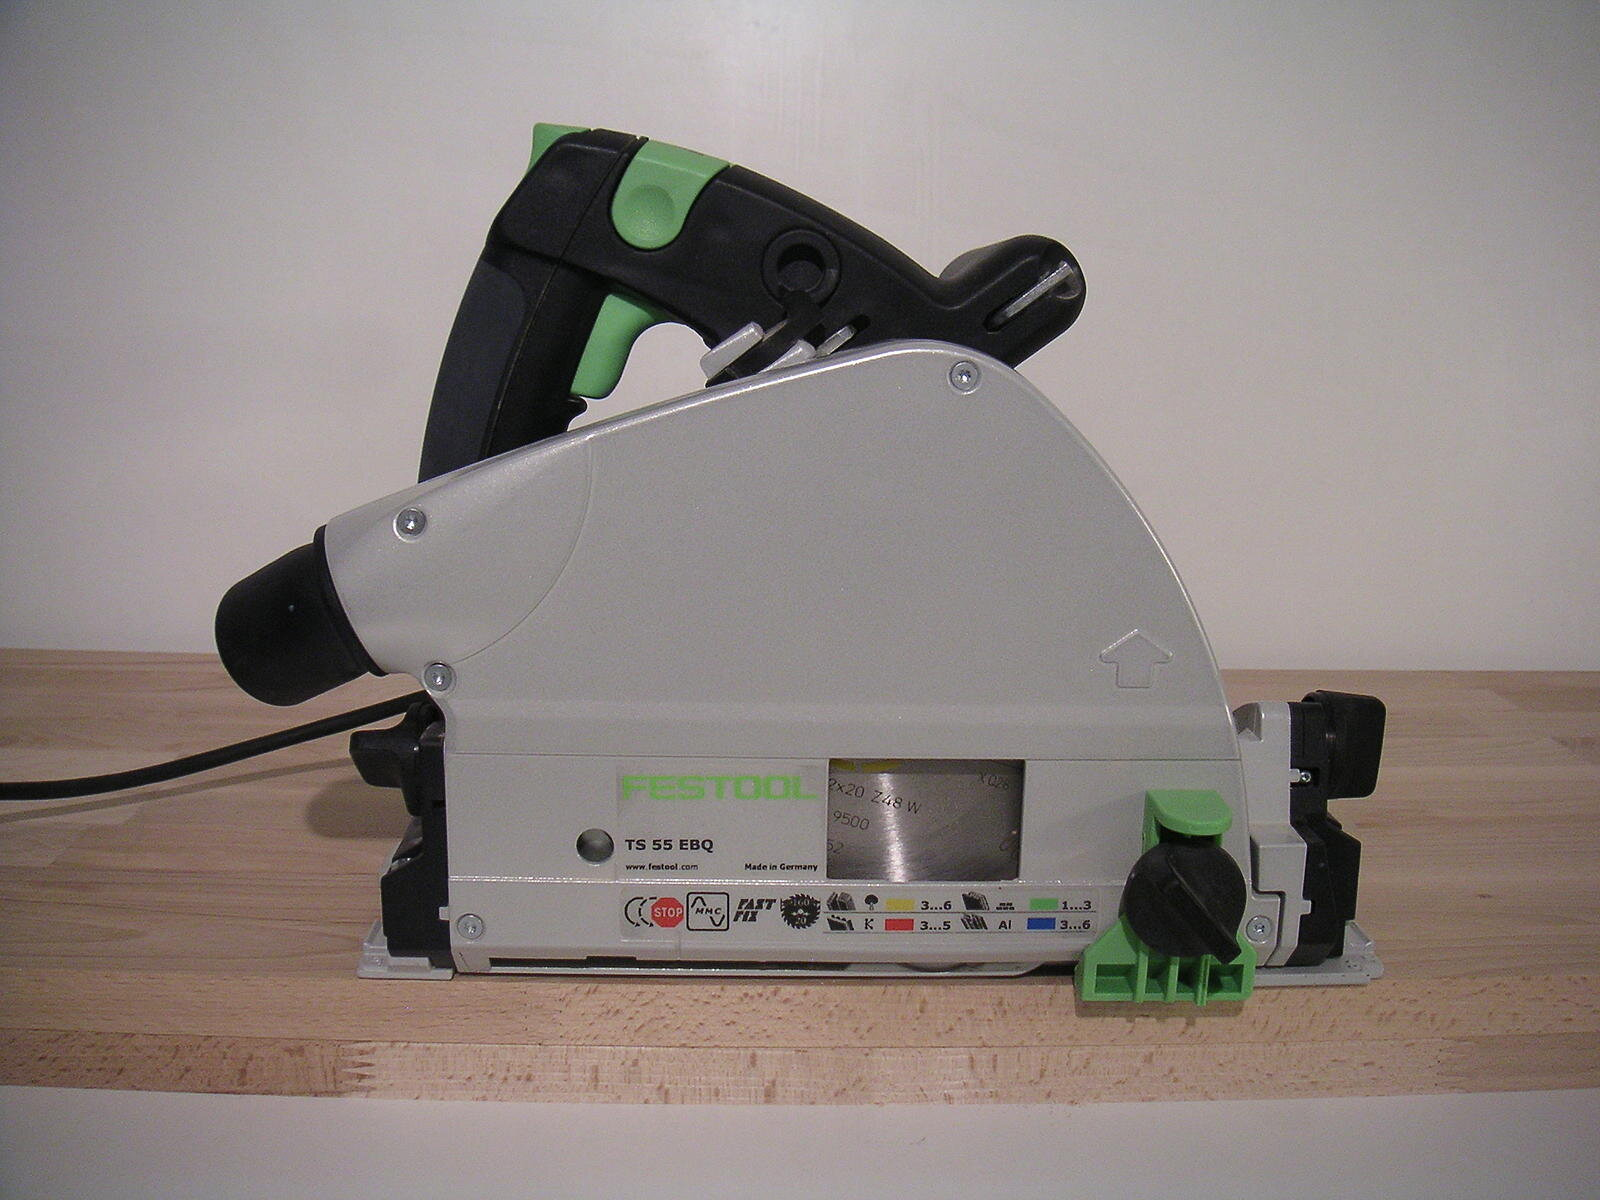
\includegraphics[width=0.49\textwidth]{bilder/ts55ebq-grundstellung.jpg}};
  \node[anchor=south west, inner sep=0pt] (b) at ([xshift=0.01\textwidth]a.south east)
    {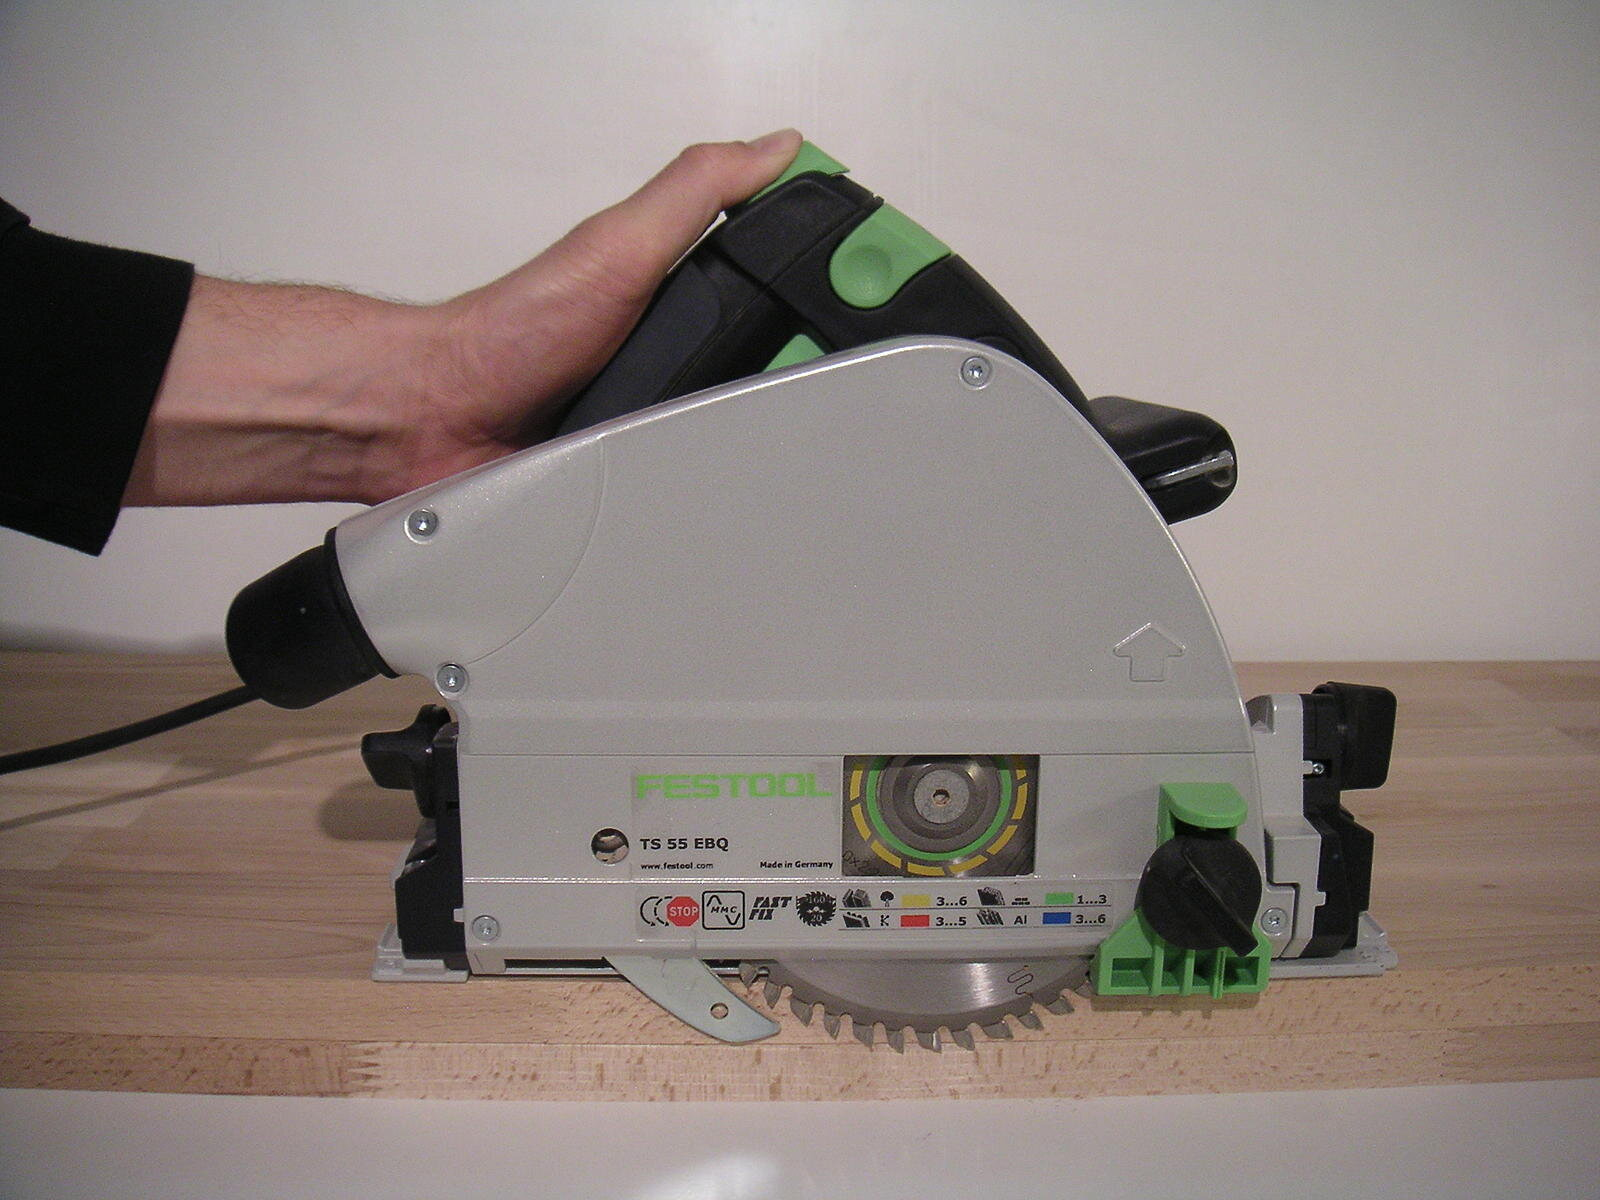
\includegraphics[width=0.49\textwidth]{bilder/ts55ebq-eingetaucht.jpg}};

  \begin{scope}[shift={(a.south west)}, x={(a.south east)}, y={(a.north west)}]
    \node[titel] at (0,1) {Grundstellung};
    \nr{1}{0.20,0.84}{0.29,0.66}
    \nr{2}{0.49,0.93}{0.405,0.83}
    \nr{3}{0.17,0.71}{0.343,0.705}
    \nr{4}{0.80,0.86}{0.64,0.76}
    \nr{5}{0.07,0.36}{0.175,0.50}
    \nr{6}{0.92,0.20}{0.745,0.255}
    \nr{7}{0.45,0.67}{0.48,0.55}
    \nr{8}{0.30,0.10}{0.40,0.205}
  \end{scope}
  \begin{scope}[shift={(b.south west)}, x={($(b.south east)-(b.south west)$)}, y={($(b.north west)-(b.south west)$)}]
    \node[titel] at (0,1) {eingetaucht};
    \nr{9}{0.72,0.09}{0.60,0.14}
    \nr{10}{0.28,0.09}{0.43,0.17}
  \end{scope}
\end{tikzpicture}
